\section{Preprocesamiento}

Antes de trabajar con los datos tenemos que aplicar cierto preprocesamiento para que se comporten de forma adecuada con el modelo que intentará predecir la clase.


La primera transformación que aplicaremos será una normalización. Debido a que los datos están en rangos de valores muy distintos y algunas de las técnicas que utilizaremos tendrán en cuenta valores como las distancias, es necesario escalar los datos para que no dar más importancia a un predictor simplemente porque sus valores son más grandes que los del resto.

Para aplicar esta transformación utilizaremos una normalización de media cero y desviación uno aplicando el método \texttt{StandardScaler} de scikit-learn.

Tras esta normalización pasaremos a aplicar el análisis de componentes principales con el método \texttt{PCA} disponible en scikit-learn. De cara a buscar un mejor espacio para la clasificación, se ha pasado como parámetro a este modelo que mantenga los suficientes datos como para explicar el 90\% de la varianza, obteniendo como resultado dieciséis nuevos predictores.

De cara a visualizar el resultado se ha creado una gráfica donde se visualiza la clase de las observaciones dependiendo de los dos nuevos predictores que más varianza explican, un poco más del 20\%:

\begin{figure}[H]
	\centering
	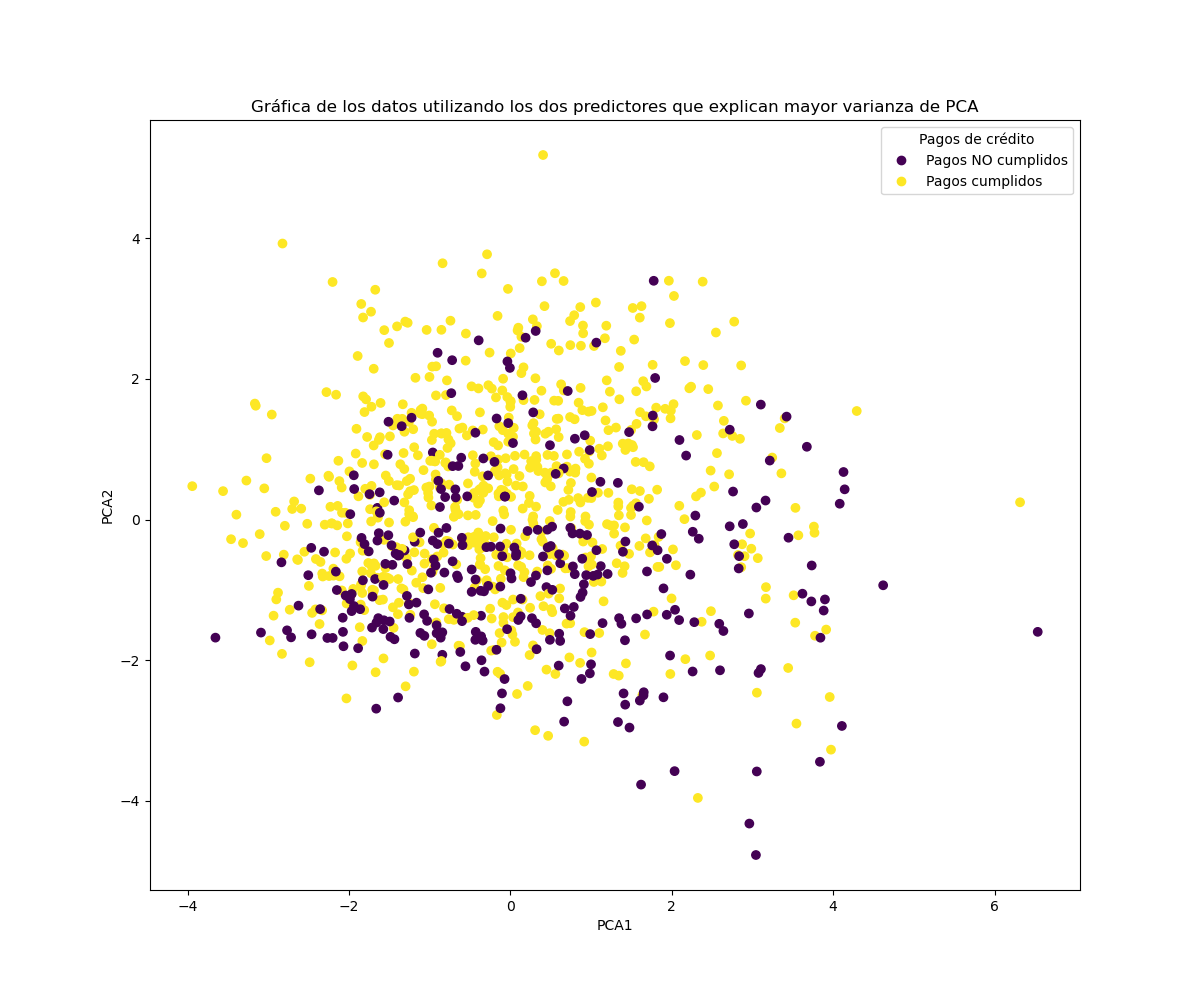
\includegraphics[scale = 0.6]{datos_pca.png}
	\caption{Observaciones en función de los dos mejores predictores tras PCA.}
	\label{fig:datos_pca}
\end{figure}

Como vemos sigue existiendo demasiado solape como para ver una distinción clara entre las clases, sin embargo esto es solo utilizando dos de los dieciséis predictores obtenidos por PCA.

\newpage
